%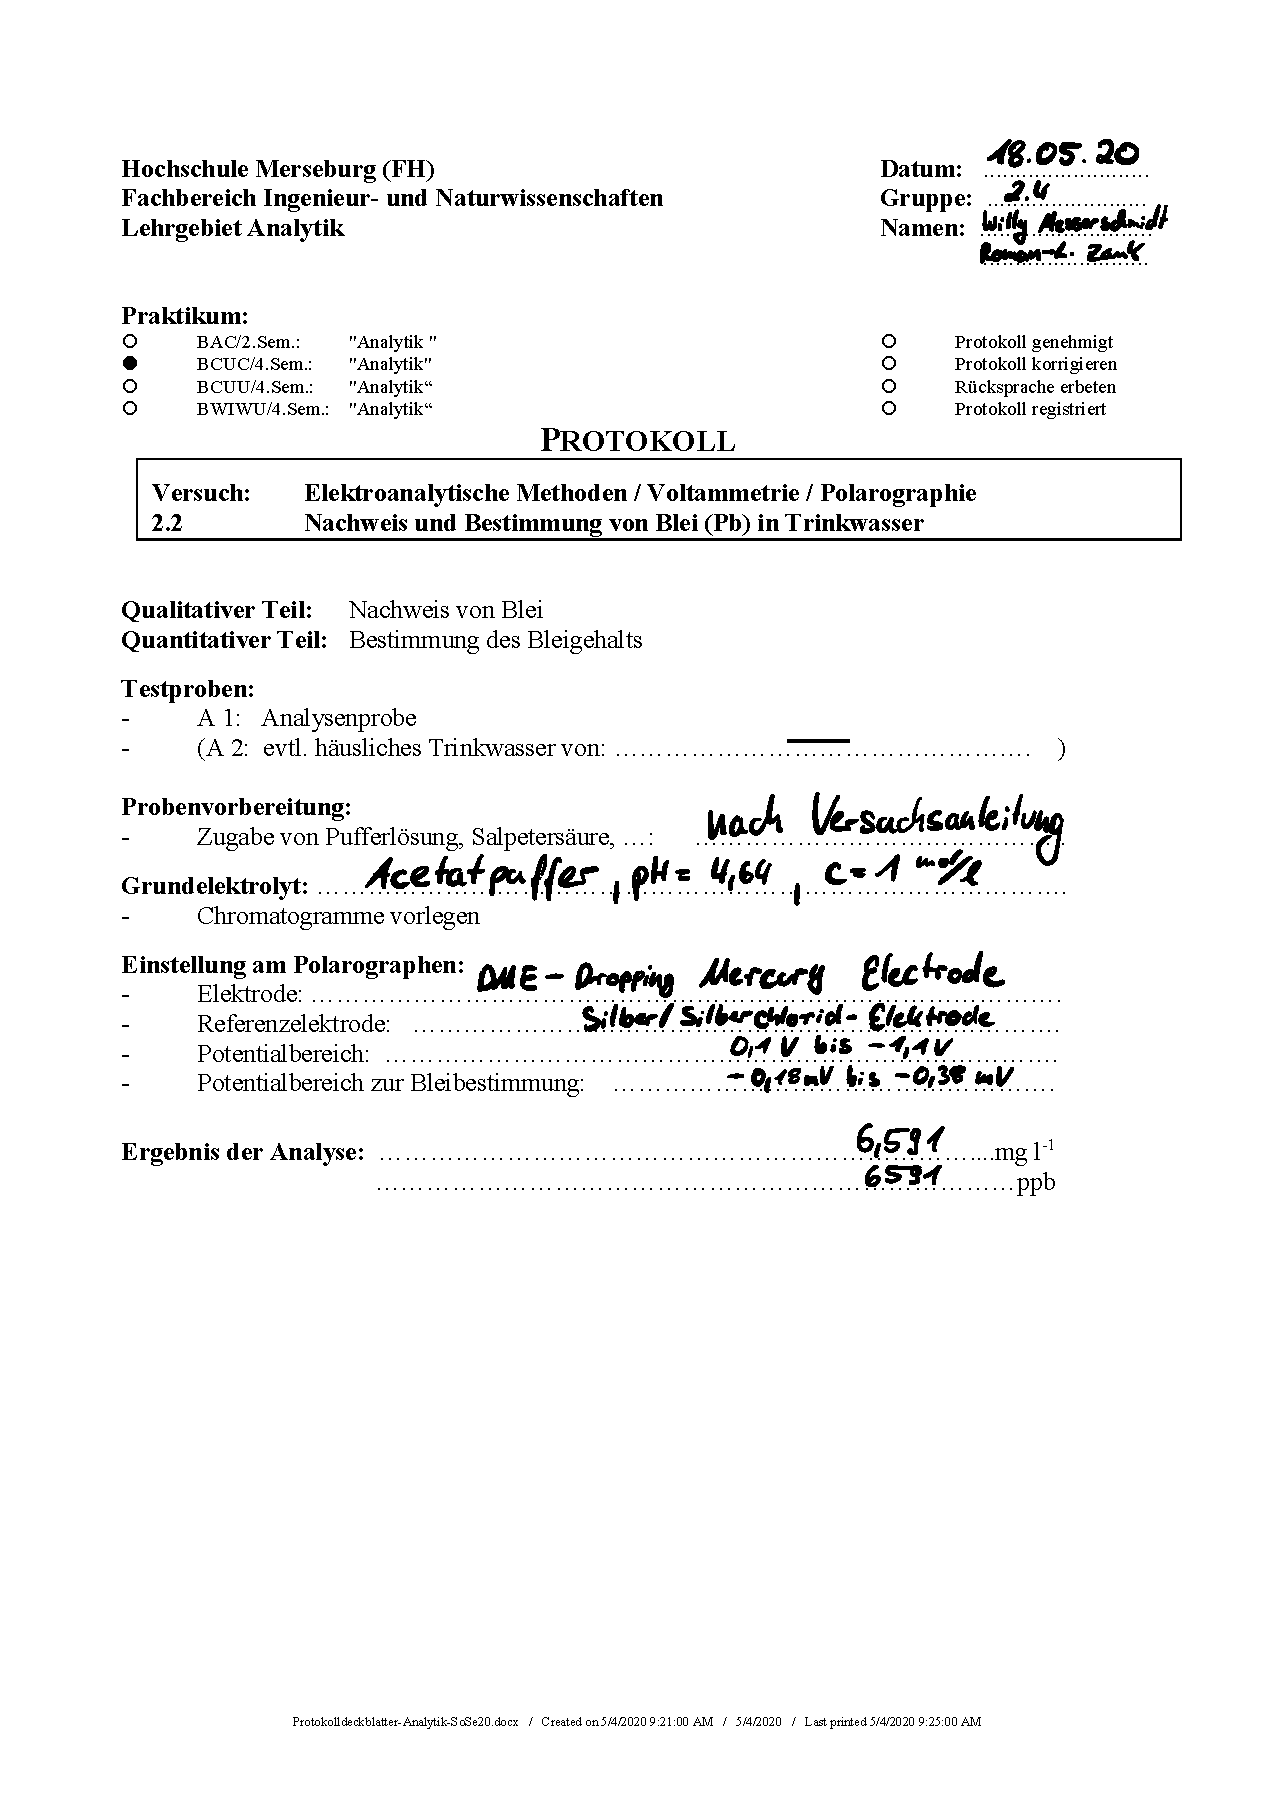
\includepdf[]{Deckblatt}
\pagebreak
\section{Einleitung}
\label{sec:einleitung}
Im folgenden Protokoll werden generierte Messdaten zum Versuch \textit{WÜK} ausgewertet. Ziel ist es mithilfe der erklärenden Videos zum Praktikum und Mittels der gegebenen Messdaten den Wärmeübergangskoeffizient $\alpha_L$ für turbulente Luftströmungen zu bestimmen. Dafür werden  drei verschiedene Rohre unter unterschiedlichen Volumenströmen der Luft untersucht. Die Wärmeübertragung mit Wasser erfolgt  in diesem Versuch mittels Gegenstrom.
Darüber hinaus sind, mittels \textsc{Nußelt}-Zahl $Nu$ und der \textsc{Nußelt}-Parameter $a$ und $b$, Bewertungen zur Wärmeübertragung der verschiedenen Rohre und Volumenströme abzugeben.





